% ══════════════════════════════════════════════════════
% PHẦN 3 — Thực nghiệm, Phân tích, Kết luận   (SƯỜN — chờ kết quả chạy chính thức trên Kaggle)
% Người thuyết trình: C (TV5 — Lương Huỳnh Gia Bảo)
% Thời lượng: ~10 phút (10 slide nội dung, ~1 phút/slide)
% ══════════════════════════════════════════════════════
%
% Mạch trình bày: kết quả chính (dị tính → đồng tính/đồ thị → tái lập) → phân tích → Key findings → kết luận.
%
% Quy ước: nhóm chỉ chạy lại DGMAE (code C:/DGMAE/DGMAE-REIMPL, chạy trên Kaggle, 10 seed 0–9);
%   số của mọi phương pháp khác lấy từ paper. Ô của nhóm tô đỏ (\nh), dòng DGMAE của paper in đậm (\dg).
% Trình bày: 1 cột; chỉ chia 2 cột khi hai bên cân nhau (cùng rộng, cùng loại nội dung).
%   Mỗi slide: 1 bảng/hình + 1 dòng kết luận (\ketluan) dạng "Paper: … · Nhóm: …"; chi tiết để ở "Lời thoại".
% [ĐIỀN] = chờ kết quả chính thức · [KIỂM TRA] = cần đối chiếu lại với paper.
%
% Slide nào lấy số từ nhóm chạy Kaggle nào (GROUP trong kaggle/run_on_kaggle.ipynb):
%   Phân loại dị tính, Phân cụm  ← main_small, main_mid, main_roman
%   Đồng tính & đồ thị           ← main_small, main_mid (Cora/Citeseer/Pubmed) · graph (Table 9)
%   Tái lập (biểu đồ)            ← vẽ lại: python scripts/plot_paper_vs_team.py
%   Ablation                     ← ablation (+ bản đầy đủ từ main_small)
%   Độ nhạy λ                    ← lambda (+ λ theo Table 8 từ main_small)

% ── Macro dùng riêng trong phần 3 ──
\newcommand{\dg}[1]{\textbf{#1}}                                  % ô của dòng DGMAE (paper): đen đậm
\newcommand{\nh}[1]{\textcolor{Theme_Color}{#1}}                  % ô của nhóm chạy lại: đỏ (khớp biểu đồ)
\newcommand{\pmstd}[1]{{\tiny$\pm$#1}}                            % std nhỏ
\newcommand{\dien}{\nh{[ĐIỀN]}}                                   % ô kết quả nhóm chưa có
\newcommand{\ketluan}[1]{%
  \vfill
  \begin{center}
    \colorbox{RiverLight}{\parbox{0.94\textwidth}{\centering\small\vspace{0.35em}#1\vspace{0.35em}}}
  \end{center}}
\newcommand{\hinhcho}[3]{%                                         % khung giữ chỗ cho hình chưa có: {rộng}{cao}{nội dung}
  \tikz\node[draw=gray!60, dashed, rounded corners, minimum width=#1, minimum height=#2,
             align=center, text=gray, font=\small]{#3};}

\section{Experiments}

% ── Slide: Thiết lập thực nghiệm ─────────────────────
\begin{frame}{Experimental Setup}
  \centering
  \textbf{Self-supervised} pre-training $\rightarrow$ frozen encoder $\rightarrow$ evaluate embeddings (Sec.~5.3)\\[1em]
  \renewcommand{\arraystretch}{1.4}
  \begin{tabular}{l l l}
    \toprule
    \textbf{Task} & \textbf{Datasets} & \textbf{Evaluation} \\
    \midrule
    Node classification  & 7 heterophilic, 3 homophilic graphs & Logistic regression \\
    Node clustering      & 6 heterophilic graphs               & K-means \\
    Graph classification & MUTAG, PROTEINS, IMDB-M, COLLAB     & SVM (10-fold CV) \\
    \bottomrule
  \end{tabular}
  \ketluan{We re-run \textbf{DGMAE only} (10 seeds, hyper-parameters from Table~8, Kaggle GPU) ·
    baselines: \textbf{numbers reported in the paper}}
  % Lời thoại:
  % - Dị tính: Texas, Cornell, Wisconsin, Chameleon, Squirrel, Actor, Roman-empire. Đồng tính: Cora, Citeseer, Pubmed.
  % - Giao thức chuẩn của học biểu diễn tự giám sát: encoder học không nhãn rồi đóng băng; chất lượng embedding
  %   đo bằng một mô hình đơn giản đặt lên trên (linear probing). Báo cáo mean ± std của 10 lần chạy.
  % - Split: Planetoid public; dị tính 10 split Geom-GCN (48/32/20); Roman 10 split (50/25/25).
  % - Code cài lại từ đầu (PyTorch, GAT tự viết), không dùng code tác giả. GPU Kaggle [ĐIỀN: P100/T4] (paper: TITAN RTX 24 GB).
  % - Paper không nêu hidden size, số head, số epoch, tiền xử lý, cấu hình linear probe → nhóm lấy theo config tác giả;
  %   linear probe: Adam, lr 0.01, wd 1e-4, 300 epoch, chọn epoch theo tập val.
  % - Không chạy: Crocodile, Amazon, Coauthor, WikiCS, Flickr và 5 đồ thị lớn ở Table 11 (thời gian, GPU).
\end{frame}

% ── Slide: Phân loại node — dị tính (Table 1) ────────
\begin{frame}{Node Classification on Heterophilic Graphs}
  \centering
  \resizebox{0.96\textwidth}{!}{%
    \begin{tabular}{ll ccccccc}
      \toprule
      & \textbf{Method} & \textbf{Texas} & \textbf{Cornell} & \textbf{Wisconsin} & \textbf{Chameleon} & \textbf{Squirrel} & \textbf{Actor} & \textbf{Roman} \\
      \midrule
      \multirow{3}{*}{Contrastive}
        & GREET    & \underline{82.70} & 73.78 & \underline{82.94} & 63.64 & 42.29 & \underline{36.55} & 50.69 \\
        & SP-GCL   & 80.36 & \underline{78.33} & 78.26 & 65.28 & 52.10 & 28.94 & 70.88 \\
        & GraphACL & 71.08 & 59.33 & 69.22 & 69.12 & 54.05 & 30.03 & \underline{74.91} \\
      \midrule
      \multirow{3}{*}{Generative}
        & NWR-GAE  & 69.62 & 58.64 & 68.23 & 72.04 & \underline{64.81} & 30.17 & 46.35 \\
        & AUG-MAE  & 72.97 & 65.14 & 76.47 & \underline{72.19} & 53.23 & 26.36 & 51.13 \\
        & GraphMAE & 55.14 & 51.62 & 55.69 & 68.67 & 44.91 & 25.61 & 46.73 \\
      \midrule
      & \dg{DGMAE (paper)}
        & \dg{88.11}\pmstd{5.16} & \dg{78.65}\pmstd{4.59} & \dg{88.43}\pmstd{3.56} & \dg{75.50}\pmstd{1.17}
        & \dg{72.47}\pmstd{1.77} & \dg{36.61}\pmstd{0.74} & \dg{76.62}\pmstd{0.41} \\
      & \nh{DGMAE (repro.)} & \dien & \dien & \dien & \dien & \dien & \dien & \dien \\
      \bottomrule
    \end{tabular}%
  }\\[0.3em]
  {\scriptsize Accuracy (\%). Baselines from Table~1 of the paper; \underline{underline}: runner-up.}
  \ketluan{Paper: DGMAE \textbf{ranks 1st on all 7 datasets} · Reproduced: [ĐIỀN: hạng 1 ở bao nhiêu dataset?]}
  % Lời thoại:
  % - Bảng chỉ giữ các phương pháp đứng thứ hai ở ít nhất một dataset (và GraphMAE để so sánh).
  %   Std của các phương pháp khác xem Table 1 của paper.
  % - Paper kết luận: DGMAE vượt cả các phương pháp contrastive thiết kế riêng cho đồ thị dị tính
  %   → L_d giải quyết được vấn đề đồng nhất hóa của GMAE.
  % - Nhóm: [ĐIỀN: so số của nhóm với các baseline của paper — thua phương pháp nào, ở dataset nào].
\end{frame}

% ── Slide: Phân cụm node (Table 3) ───────────────────
\begin{frame}{Node Clustering on Heterophilic Graphs}
  \centering
  \resizebox{0.96\textwidth}{!}{%
    \begin{tabular}{ll cccccc}
      \toprule
      & \textbf{Method} & \textbf{Texas} & \textbf{Cornell} & \textbf{Wisconsin} & \textbf{Chameleon} & \textbf{Squirrel} & \textbf{Roman} \\
      \midrule
      \multirow{4}{*}{ACC}
        & GREET    & 52.40 & 48.96 & 56.65 & 34.44 & 25.64 & 31.43 \\
        & GraphMAE & 46.28 & 46.12 & 52.67 & 37.02 & 27.61 & 15.38 \\
        & \dg{DGMAE (paper)} & \dg{66.83}\pmstd{6.19} & \dg{57.16}\pmstd{5.99} & \dg{68.69}\pmstd{4.52} & \dg{39.96}\pmstd{1.74} & \dg{30.83}\pmstd{0.71} & \dg{36.25}\pmstd{0.86} \\
        & \nh{DGMAE (repro.)}  & \dien & \dien & \dien & \dien & \dien & \dien \\
      \midrule
      \multirow{4}{*}{NMI}
        & GREET    & 37.19 & 28.19 & 22.57 & 14.99 &  3.22 & 37.00 \\
        & GraphMAE &  6.06 & 12.07 & 18.54 & 19.47 &  4.58 &  9.33 \\
        & \dg{DGMAE (paper)} & \dg{37.41}\pmstd{7.20} & \dg{34.41}\pmstd{7.88} & \dg{44.19}\pmstd{2.19} & \dg{22.39}\pmstd{0.43} & \dg{8.00}\pmstd{0.73} & \dg{37.57}\pmstd{0.53} \\
        & \nh{DGMAE (repro.)}  & \dien & \dien & \dien & \dien & \dien & \dien \\
      \bottomrule
    \end{tabular}%
  }\\[0.3em]
  {\scriptsize K-means on embeddings (\%). GREET, GraphMAE from Table~3 of the paper; ARI and F1 show the same trend.}
  \ketluan{Paper: DGMAE \textbf{ranks 1st in all 24 cells} (6 datasets $\times$ 4 metrics) · Reproduced: [ĐIỀN]}
  % Lời thoại:
  % - Phân cụm khó hơn phân loại vì không dùng nhãn nào. GraphMAE gần như "mù" trên Texas (NMI 6, ARI ~1).
  % - Paper: cách biệt lớn nhất ở ARI (Texas +18.0, Wisconsin +19.2 so với GREET).
  % - Hạng 2 ở Texas ACC là NWR-GAE (55.03); ở Squirrel F1 là MaskGAE (23.27); các ô còn lại là GREET hoặc GraphMAE.
  % - Nhóm (ARI, F1 — không đưa lên slide): [ĐIỀN].
\end{frame}

% ── Slide: Đồng tính (Table 2) & phân loại đồ thị (Table 9) — 2 cột cân nhau: mỗi bên 4 baseline + 2 dòng DGMAE ──
\begin{frame}{Homophilic Graphs \& Graph Classification}
  \begin{columns}[t]
    \begin{column}{0.48\textwidth}
      \centering
      {\small\textbf{Node classification — Table~2}}\\[0.4em]
      {\scriptsize\setlength{\tabcolsep}{3pt}
      \begin{tabular}{l ccc}
        \toprule
        \textbf{Method} & \textbf{Cora} & \textbf{Citeseer} & \textbf{Pubmed} \\
        \midrule
        GraphACL & 84.20 & \underline{73.63} & 82.02 \\
        NWR-GAE  & 83.62 & 71.45 & \underline{83.44} \\
        Bandana  & \underline{84.62} & 73.60 & \textbf{83.53} \\
        GraphMAE & 84.20 & 73.40 & 81.10 \\
        \midrule
        \dg{DGMAE (paper)} & \dg{84.93}\pmstd{0.51} & \dg{73.82}\pmstd{0.64} & 81.10\pmstd{0.42} \\
        \nh{DGMAE (repro.)}  & \dien & \dien & \dien \\
        \bottomrule
      \end{tabular}}
    \end{column}
    \begin{column}{0.48\textwidth}
      \centering
      {\small\textbf{Graph classification — Table~9}}\\[0.4em]
      {\scriptsize\setlength{\tabcolsep}{3pt}
      \begin{tabular}{l cccc}
        \toprule
        \textbf{Method} & \textbf{MUTAG} & \textbf{PROTEINS} & \textbf{IMDB-M} & \textbf{COLLAB} \\
        \midrule
        Infograph & \underline{89.01} & 74.44 & 49.69 & 70.65 \\
        S2GAE     & 88.26 & \underline{76.37} & 51.79 & \underline{81.02} \\
        AUG-MAE   & 88.28 & 75.83 & \underline{51.80} & 80.48 \\
        GraphMAE  & 88.19 & 75.30 & 51.63 & 80.32 \\
        \midrule
        \dg{DGMAE (paper)} & \dg{89.06}\pmstd{0.64} & \dg{76.51}\pmstd{0.52} & \dg{51.95}\pmstd{0.30} & \dg{81.15}\pmstd{0.30} \\
        \nh{DGMAE (repro.)}  & \dien & \dien & \dien & \dien \\
        \bottomrule
      \end{tabular}}
    \end{column}
  \end{columns}
  \vspace{0.5em}
  \centering{\scriptsize Accuracy (\%). Baselines from the paper; \underline{underline}: runner-up.}
  \ketluan{Paper: 1st on Cora, Citeseer and all 4 graph datasets $\Rightarrow$ $\mathcal{L}_d$ \textbf{does not hurt} · Reproduced: [ĐIỀN]}
  % Lời thoại:
  % - DGMAE được thiết kế cho đồ thị dị tính; ở đây paper chỉ cần chứng minh "không làm hại".
  % - Table 2 trên slide chỉ giữ phương pháp hạng 2 / tốt nhất ở ít nhất một dataset và GraphMAE
  %   (GREET 83.82/73.22/80.20, AUG-MAE 84.30/73.20/81.12 — xem Table 2 của paper).
  % - Pubmed: DGMAE của paper bằng GraphMAE (81.10), không đứng đầu (Bandana 83.53 tốt nhất — in đậm).
  % - Phân loại đồ thị: encoder GIN; L_d dùng L_sym X (Eq. 5). Table 8 không có siêu tham số cho tác vụ này → theo config tác giả.
  % - Nhóm: [ĐIỀN].
\end{frame}

% ── Slide: Tái lập: nhóm vs. paper ───────────────────
\begin{frame}{Reproducibility: Reproduced vs.\ Paper}
  \centering
  % Khi có kết quả: chạy  python scripts/plot_paper_vs_team.py  (trong DGMAE-REIMPL), rồi thay khung dưới bằng:
  %   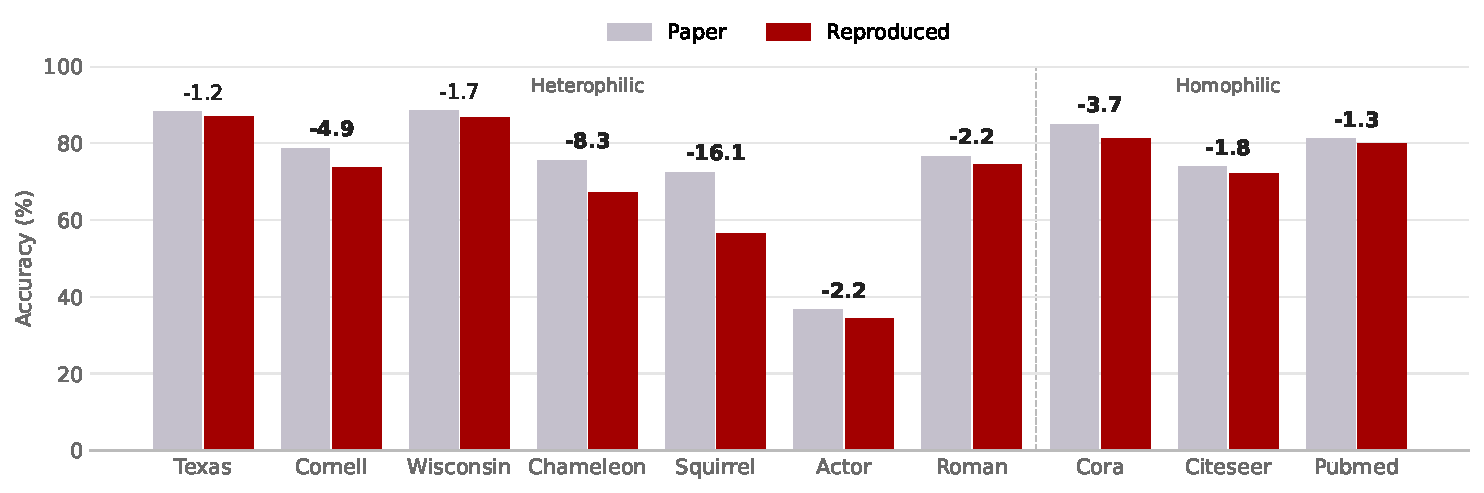
\includegraphics[width=\textwidth]{paper_vs_nhom.pdf}
  \hinhcho{0.95\textwidth}{0.52\textheight}{[ĐIỀN] Bar chart: DGMAE accuracy, paper vs.\ reproduced, 10 datasets\\
    (label: reproduced $-$ paper; bold if outside 1 std)}\\[0.1em]
  {\scriptsize DGMAE node classification accuracy. Labels: reproduced $-$ paper; \textbf{bold}: outside 1 std of the paper.}
  \ketluan{[ĐIỀN: bao nhiêu dataset nằm trong 1 std · chênh lệch trung bình dị tính / đồng tính]}
  % Lời thoại:
  % - Chênh lệch trung bình: dị tính [ĐIỀN] · đồng tính [ĐIỀN] · phân cụm (NMI) [ĐIỀN].
  % - Nguyên nhân có thể (kiểm tra lại khi có số chính thức): paper thiếu cấu hình (hidden size, số head, số epoch,
  %   tiền xử lý, linear probe); Table 8 khác config của tác giả (ví dụ Cora: lr 1e-4 trong paper, 1e-3 trong code —
  %   nhóm theo paper); phân cụm: code tác giả gán cứng λ = 0.4/0.6, không có trong Table 8.
  % - Code tác giả chọn epoch theo tập test, nhóm chọn theo tập val.
  % - Chi phí: Roman [ĐIỀN] MB, [ĐIỀN] s/vòng trên GPU Kaggle; paper (TITAN RTX): 1 416 MB, 1.50 s/vòng.
\end{frame}

\section{Analysis}

% ── Slide: Ablation (Table 4) ────────────────────────
\begin{frame}{Ablation Study}
  \centering
  \resizebox{0.80\textwidth}{!}{%
    \begin{tabular}{l c cc cc}
      \toprule
      & \textbf{Roman} & \multicolumn{2}{c}{\textbf{Actor}} & \multicolumn{2}{c}{\textbf{Citeseer}} \\
      \cmidrule(lr){2-2} \cmidrule(lr){3-4} \cmidrule(lr){5-6}
      \textbf{Variant} & Paper & Paper & \nh{Repro.} & Paper & \nh{Repro.} \\
      \midrule
      w/o adaptive edge selection                        & 75.35          & 33.41          & \dien & 73.03          & \dien \\
      w/o $\mathcal{L}_d$ ($\approx$ GraphMAE)$^{*}$      & \textbf{36.71} & \textbf{28.14} & \dien & 73.05          & \dien \\
      w/o $\mathcal{L}_f$ ($\mathcal{L}_d$ only)$^{*}$     & 75.04          & 35.16          & \dien & \textbf{58.02} & \dien \\
      \midrule
      \dg{DGMAE (full)}                                  & \dg{76.62}     & \dg{36.61}     & \dien & \dg{73.82}     & \dien \\
      \bottomrule
    \end{tabular}%
  }\\[0.3em]
  {\scriptsize Accuracy (\%), Table~4. Bold: largest drop. $^{*}$Labels swapped in the paper; corrected using Fig.~10.
    Roman not reproduced (too costly).}
  \ketluan{Paper: w/o $\mathcal{L}_d$ loses \textbf{$\sim$40 points} on heterophilic Roman; w/o $\mathcal{L}_f$ loses 16 points on homophilic Citeseer ·
    Reproduced: [ĐIỀN: cùng xu hướng?]}
  % Lời thoại:
  % - Dị tính: L_d là cốt lõi. Đồng tính (Citeseer): bỏ L_f mất ~16 điểm → ngữ cảnh láng giềng (L_f, GraphMAE gốc) vẫn cần.
  % - Chọn cạnh thích ứng: cải thiện nhỏ nhưng đều (+0.8 đến +3.2).
  % - Vì sao biết paper ghi ngược nhãn: Fig. 10 cho λ = 0 (bỏ L_d): Roman 0.37, Actor 0.28; λ = 1 (bỏ L_f): Citeseer 0.58.
  % - Biến thể của nhóm: bỏ L_d = --lam 0 · bỏ L_f = --lam 1 · bỏ chọn cạnh = --selection all. Nhóm: [ĐIỀN].
\end{frame}

% ── Slide: Vì sao hiệu quả — chọn cạnh (Table 6) & trực quan hóa (Fig. 8) — 2 cột cân nhau ──
\begin{frame}{Why Does DGMAE Work?}
  \begin{columns}[T]
    \begin{column}{0.48\textwidth}
      \centering
      {\small\textbf{Edge selection — Table~6}}\\[0.4em]
      \resizebox{0.95\columnwidth}{!}{%
        \begin{tabular}{l ccc}
          \toprule
          \textbf{Select by} & \textbf{Actor} & \textbf{Chameleon} & \textbf{Squirrel} \\
          \midrule
          High attention ($w_{ij}$) & 34.34 & 70.88 & 58.20 \\
          Random                   & 34.72 & 71.80 & 60.07 \\
          Node degree              & 35.12 & 73.44 & 60.63 \\
          \midrule
          \dg{Low attention ($1-w_{ij}$)} & \dg{35.36} & \dg{73.90} & \dg{65.61} \\
          \bottomrule
        \end{tabular}%
      }\\[0.4em]
      {\scriptsize Low attention is best $\Rightarrow$\\ attention detects heterophilic edges}
    \end{column}
    \begin{column}{0.48\textwidth}
      \centering
      {\small\textbf{Inter-class node pairs (Roman) — Fig.~8}}\\[0.4em]
      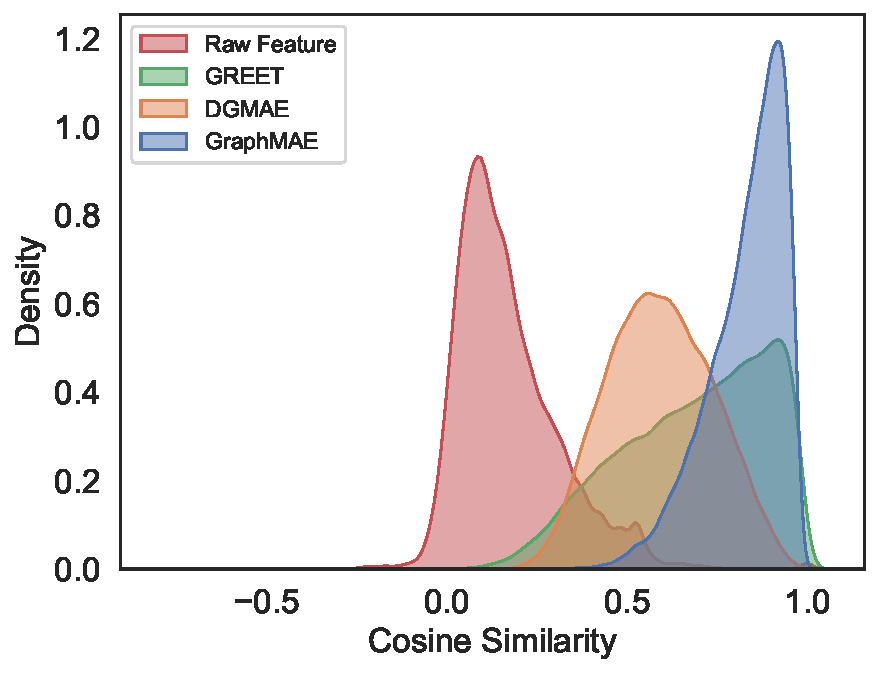
\includegraphics[height=0.40\textheight]{new_roman.pdf}\\[0.4em]
      {\scriptsize GraphMAE makes them similar ($\sim$1.0);\\ DGMAE preserves the discrepancy}
    \end{column}
  \end{columns}
  \ketluan{Attention \textbf{identifies heterophilic edges} $\Rightarrow$ DGMAE \textbf{preserves node discrepancy}}
  % Lời thoại:
  % - Số và hình trên slide này là của paper. Table 6 chỉ dùng L_d nên số thấp hơn Table 1; p_c = 0.2, p_τ = 1.
  % - Fig. 4 (ảnh hưởng của p_c): có lợi trên đồ thị dị tính, có hại trên đồ thị đồng tính.
  % - Fig. 8: cosine similarity của cặp node nối nhau nhưng khác lớp. GMAE đẩy similarity lên ~1.0 (đồng nhất hóa);
  %   DGMAE kéo về gần phân bố của đặc trưng gốc → giải quyết đúng vấn đề nêu ở Figure 2 phần mở đầu.
  % - (Tùy chọn, nếu nhóm kịp) vẽ lại Fig. 8 từ embedding của nhóm (train_node.py --save_emb).
  % - Fig. 5 (tỉ lệ che, Roman): DGMAE ổn định khi che tới 80%, GraphMAE giảm từ 46.73 xuống 38.2 — nói miệng nếu được hỏi.
\end{frame}

% ── Slide: Độ nhạy λ (Fig. 10) — 2 cột cân nhau: hình paper | hình nhóm, cùng kích thước ──
\begin{frame}{Sensitivity to $\lambda$}
  \begin{columns}[T]
    \begin{column}{0.48\textwidth}
      \centering
      {\small\textbf{Paper — Fig.~10}}\\[0.4em]
      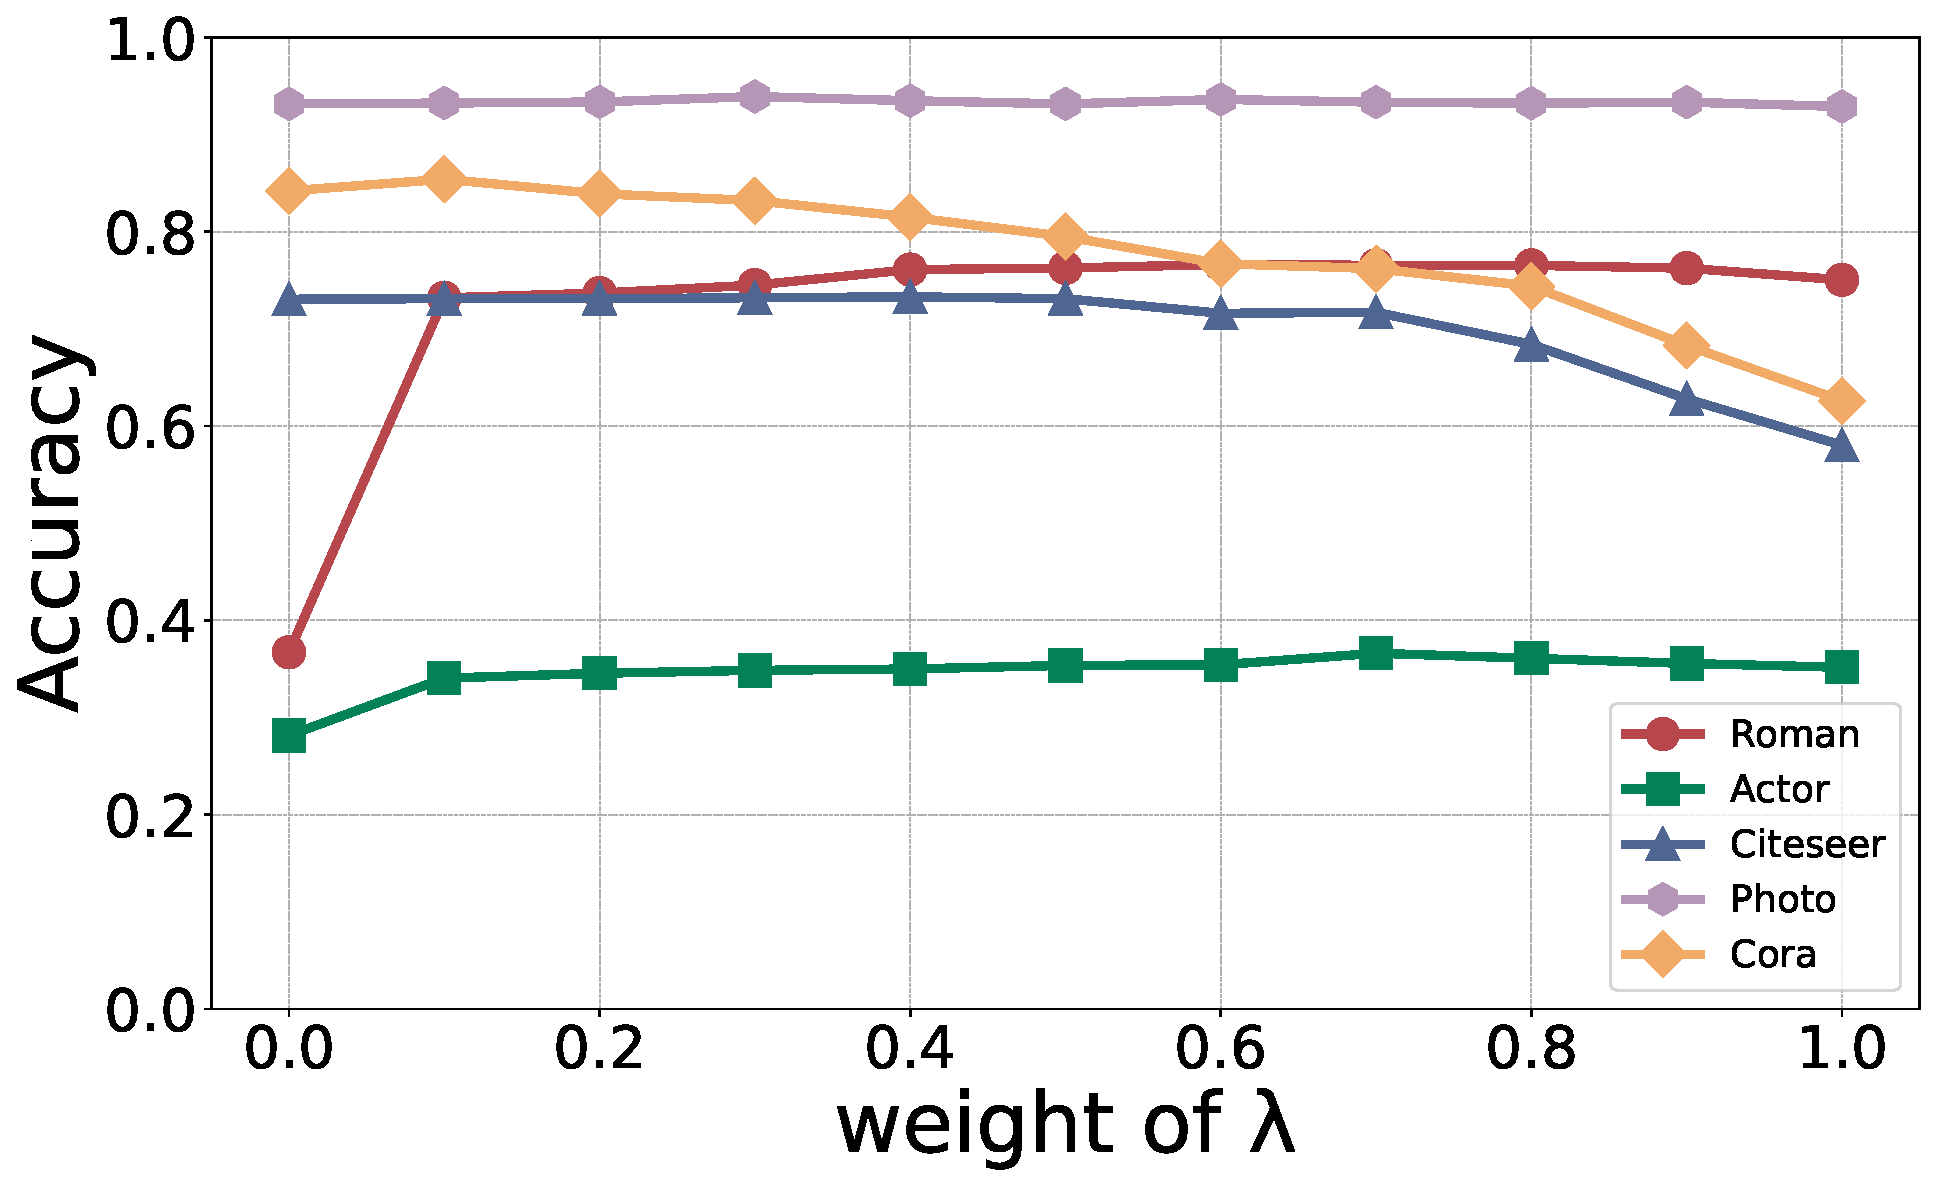
\includegraphics[height=0.45\textheight]{lambda_sens.pdf}
    \end{column}
    \begin{column}{0.48\textwidth}
      \centering
      {\small\textbf{\nh{Reproduced} — Cornell, Cora}}\\[0.4em]
      % Khi có kết quả: thay khung dưới bằng \includegraphics[height=0.45\textheight]{lambda_nhom.pdf}
      \hinhcho{0.85\linewidth}{0.45\textheight}{[ĐIỀN] Accuracy vs.\ $\lambda$\\ Cornell (heterophilic), Cora (homophilic)}
    \end{column}
  \end{columns}
  \ketluan{Paper: heterophilic graphs need large $\lambda$ (0.4--0.7), homophilic graphs small $\lambda$ ($\approx$0.1) · Reproduced: [ĐIỀN]}
  % Lời thoại:
  % - λ = 0: chỉ L_f (≈ GraphMAE); λ = 1: chỉ L_d.
  % - λ cần chọn theo mức độ dị tính của đồ thị — đây cũng là một hạn chế (thêm siêu tham số).
  % - Nhóm: [ĐIỀN]. Hình của nhóm: [ĐIỀN: script vẽ, ví dụ scripts/plot_lambda.py — chưa có].
\end{frame}

\section{Conclusion}

% ── Slide: Key findings ──────────────────────────────
\begin{frame}{Key Findings}
  \centering
  \renewcommand{\arraystretch}{1.4}
  \begin{tabular}{p{0.58\textwidth} p{0.30\textwidth}}
    \toprule
    \textbf{Finding (paper)} & \textbf{Reproduced?} \\
    \midrule
    DGMAE is best on \textbf{heterophilic graphs} (classification \& clustering) & \nh{[ĐIỀN]} \\
    \textbf{No loss} on homophilic graphs and graph classification         & \nh{[ĐIỀN]} \\
    $\mathcal{L}_d$ is the \textbf{key component} on heterophilic graphs  & \nh{[ĐIỀN]} \\
    $\lambda$ must be tuned to the heterophily level                       & \nh{[ĐIỀN]} \\
    \midrule
    \textbf{Overall reproducibility}                                        & \nh{[ĐIỀN]} \\
    \bottomrule
  \end{tabular}
  \ketluan{[ĐIỀN: một câu tổng kết — điều nhóm tin chắc nhất sau khi chạy lại]}
  % Lời thoại:
  % - Cột "Nhóm kiểm chứng": ghi ngắn, ví dụ "Có — 5/7 dataset" / "Một phần" / "Không" (điền theo số chính thức).
  % - Slide này trả lời trực tiếp yêu cầu "key findings" của đồ án.
\end{frame}

% ── Slide: Kết luận ──────────────────────────────────
\begin{frame}{Conclusion}
  \begin{itemize}
    \setlength{\itemsep}{1em}
    \item \textbf{Paper:} reconstructing the \textbf{discrepancy} $\Rightarrow$ clear gains on \textbf{heterophilic graphs},
      no loss on homophilic graphs.
    \item \textbf{Reproduction:} DGMAE re-implemented from the paper, without the authors' code. Result: [ĐIỀN: một câu tóm tắt mức độ tái lập]
    \item \textbf{Limitation:} extra hyper-parameters ($\lambda$, $p_c$, $p_\tau$, $\gamma_2$) tuned per dataset
      $\rightarrow$ future work: choose $\lambda$ \textbf{automatically} from the heterophily level.
  \end{itemize}
  \ketluan{\textbf{A simple idea that works on heterophilic graphs} — [ĐIỀN: nhận xét về tính tái lập]}
  % Lời thoại:
  % - Nhóm tái lập [ĐIỀN] tác vụ trên [ĐIỀN] dataset.
  % - Hạn chế khác của phương pháp: encoder chạy 2 lần mỗi vòng. Hướng khác: huấn luyện mini-batch cho đồ thị lớn.
  % - Hạn chế của nhóm: chưa chạy dataset lớn, chưa tái hiện Table 5, 10, 11, 12.
\end{frame}

% ── Slide cảm ơn nằm trong main.tex (\makethankyou) ──
